\section{Systemmodell}

\subsection{Systemdiagramm}

\begin{figure}[H]
    \centering
    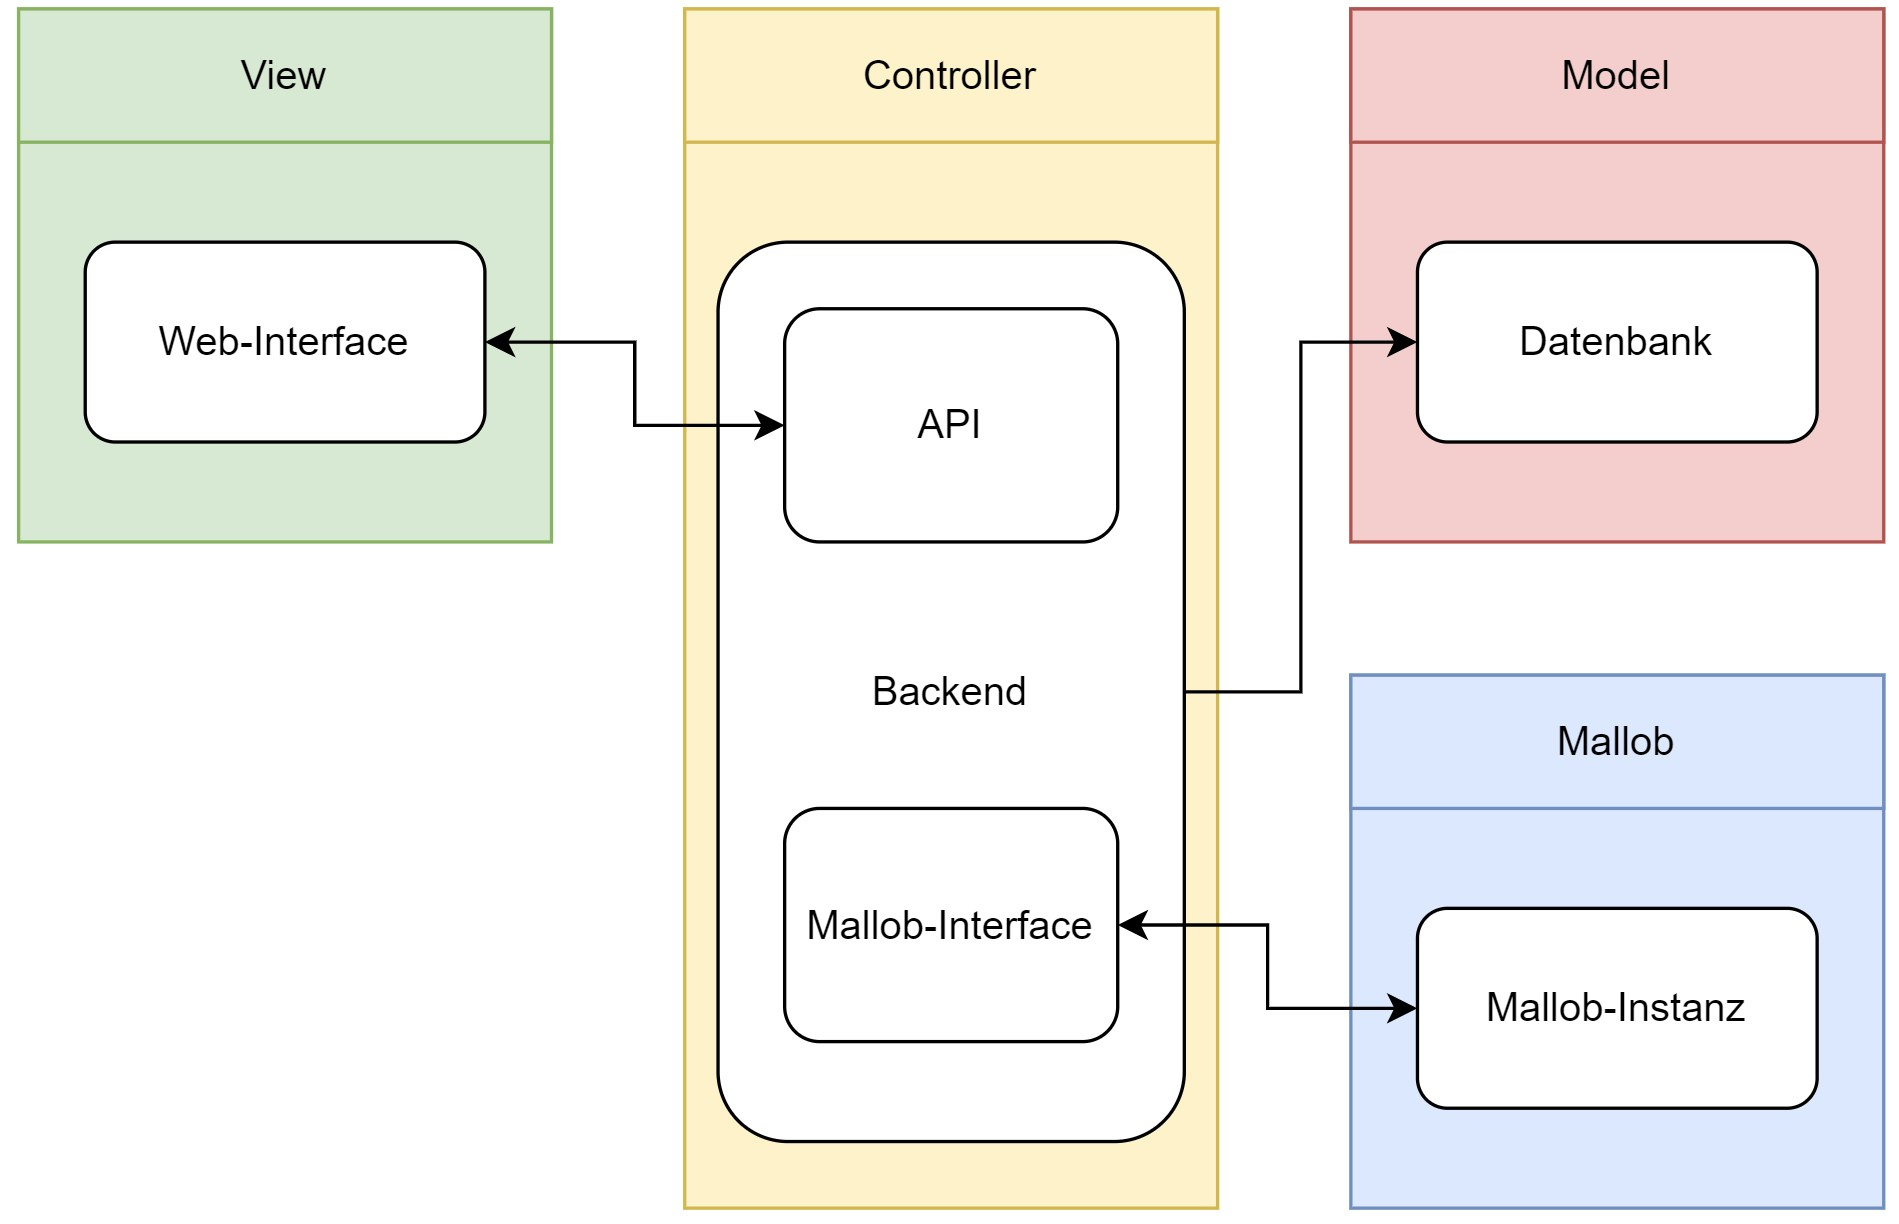
\includegraphics[width=\textwidth]{images-interface/Systemdiagramm3.jpg} \\
    \caption{Model-View-Controller}
\end{figure}
Das System kann semantisch in 3 Komponenten gegliedert werden; View, Controller sowie Model. \\
Die Aufgabe des \textbf{Views}, bzw. des Web-Interfaces ist es dabei eine interaktive, grafische Benutzeroberfläche für die Interaktion mit Mallob bereitzustellen. \\
Der \textbf{Controller}, bzw. API sowie Backend (Anfragen gehen über API an das Backend) sind für die Kommunikation zwischen Datenbank, Mallob und Web-Interface, bzw. Nutzer zuständig. Das Mallob-Interface ist im Backend implementiert und für die Kommunikation zwischen der Backend-Logik und einer laufenden Mallob-Instanz zuständig.\\
Das \textbf{Model} ist für das Bearbeiten sowie halten der Daten zuständig. Dabei hält die Datenbank die Daten des Systems (Siehe 6 Produkt-Daten [TODO verlinken]) und Mallob ist Mallob. \\
\textbf{Extern} liegt die laufende Mallob-Instanz. Mallob ist nicht Teil unseres Systems. Unser System kommuniziert lediglich mit Mallob.

\pagebreak

\subsection{Anwendungsfalldiagramme}

\begin{figure}[H]
    \centering    
    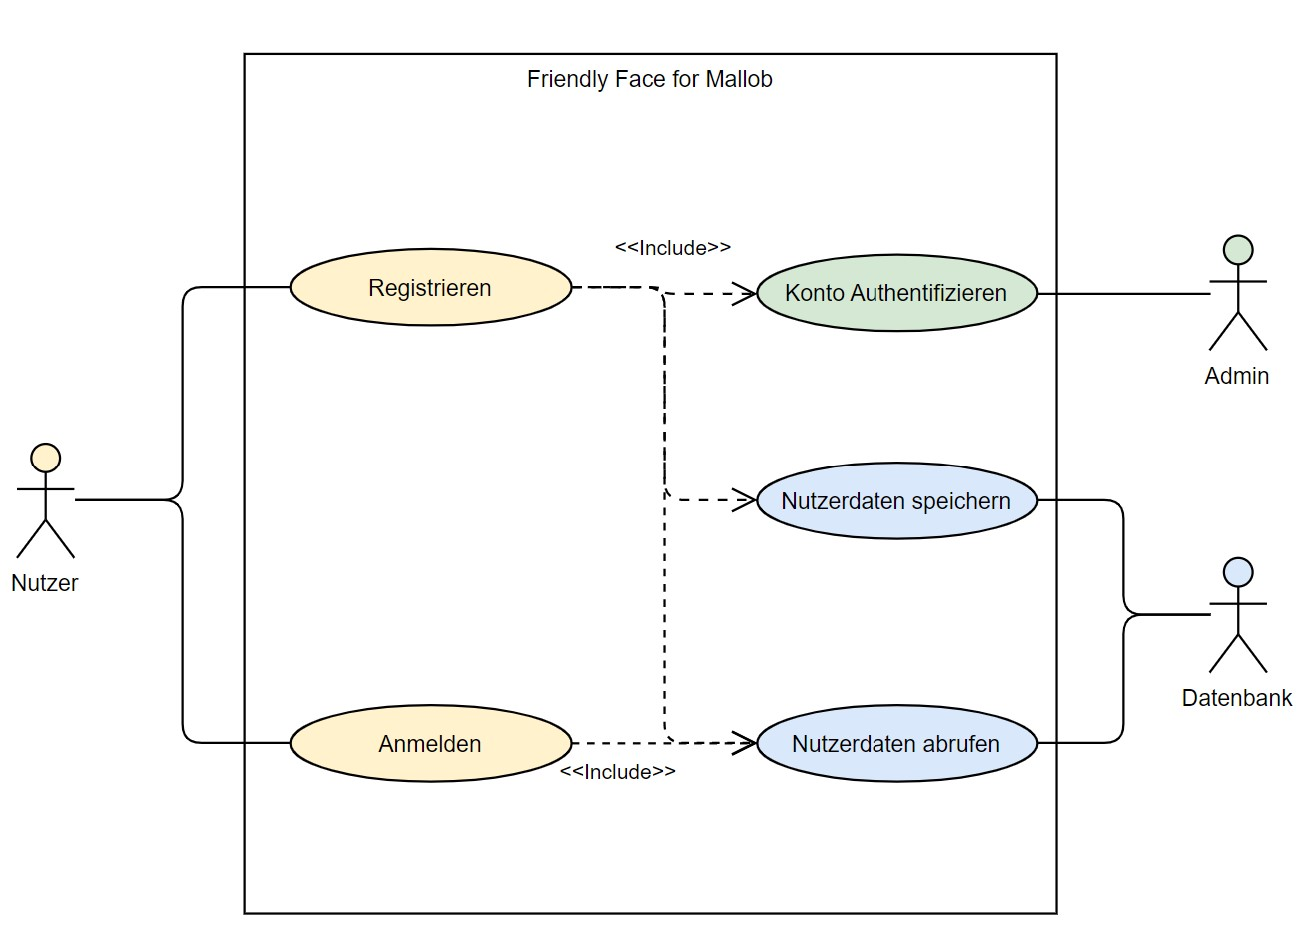
\includegraphics[width=\textwidth]{images-interface/Login_register_3_screenshot.jpg} 
    \caption{Registrierung von Nutzern}
\end{figure}


Registriert sich ein Nutzer, so wird seine Registrierunganfrage von einem Administrator verifiziert. Die Datenbank speichert die \hyperref[PD:Nutzerdaten]{Nutzerdaten}.\\
Möchte sich ein registrierter Nutzer im Web-Interface anmelden, so werden die Nutzerdaten aus der Datenbank geholt und mit den eingegebenen Daten verglichen. \\
Stellt ein registrierter Nutzer eine Anfrage über API mit seinem Token, wird auch hier der Token aus der Datenbank geholt und verglichen.
\begin{figure}[H]
    \centering
    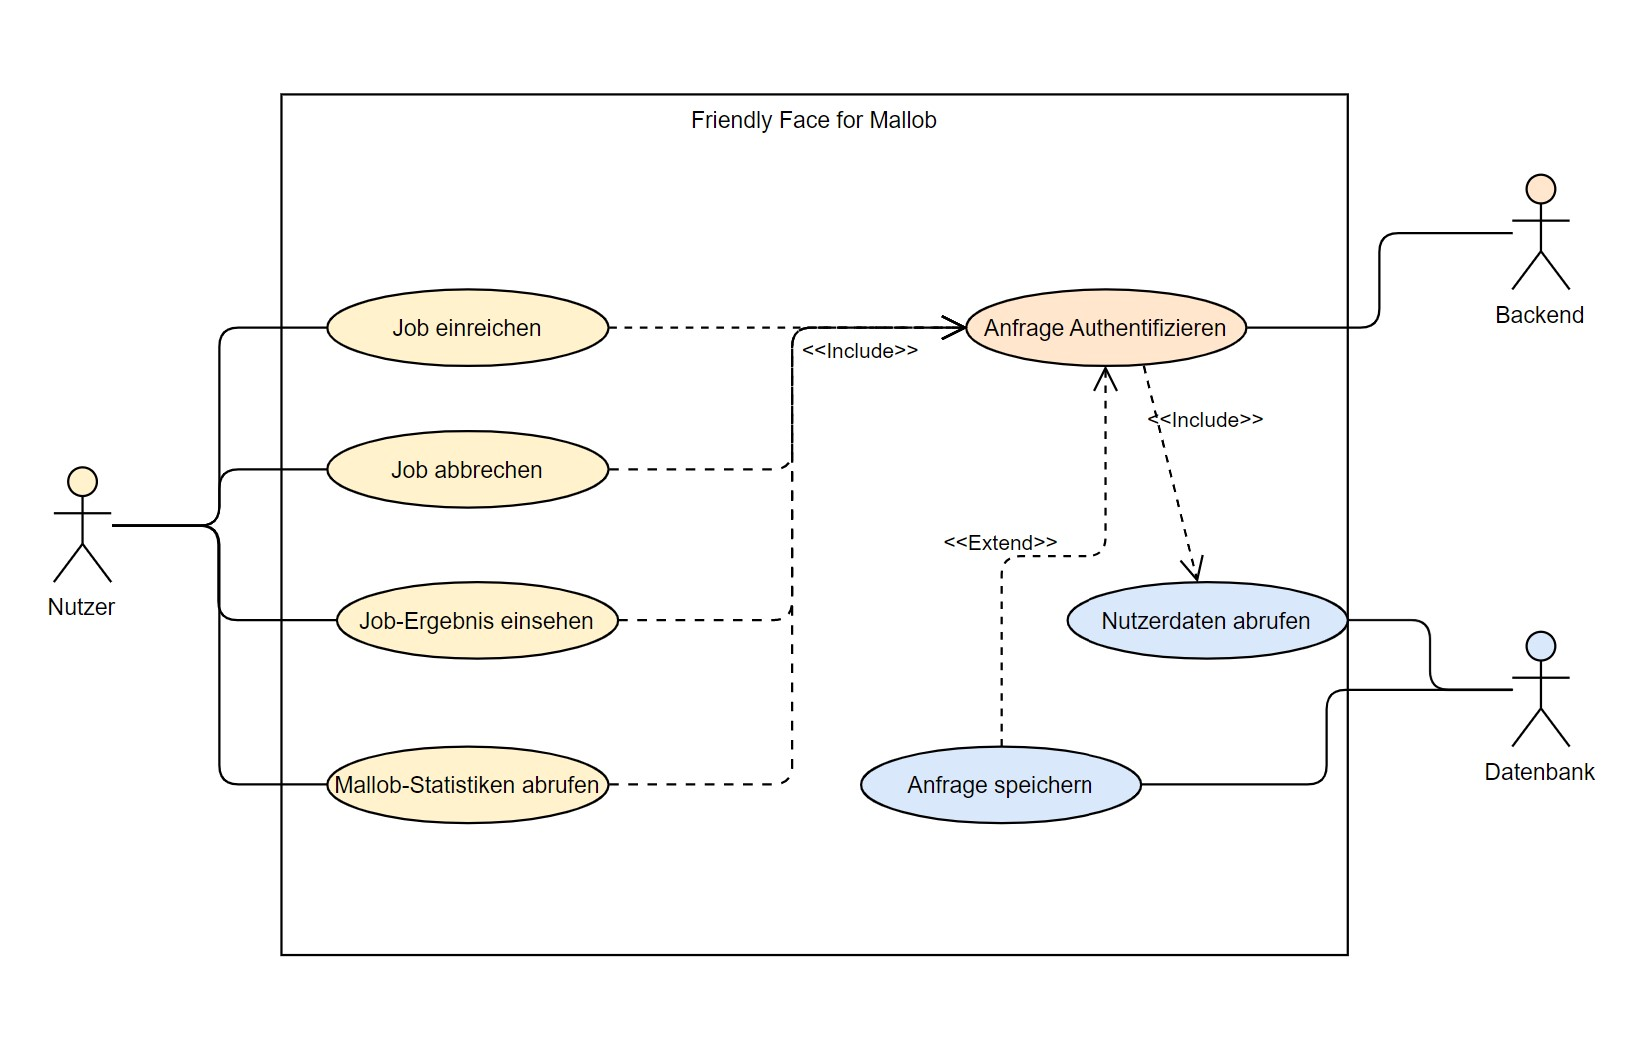
\includegraphics[width=\textwidth]{images-interface/Request_authntification_screenshot.jpg}
    \caption{Authentifizierung von API-Anfragen}
\end{figure}
Jede Anfrage an die API muss authentifiziert werden. Dies geschieht, indem der Token, der mit der Anfrage geschickt wurde, mit dem in der Datenbank gespeichertem Token abgeglichen wird. Wurde eine Anfrage verifiziert, also sichergestellt, das der Nutzer diese auch ausführen darf, so wird sie weiterverarbeitet.\\
Jede Anfrage an die API wird für eine gewisse Zeit gespeichert, um sie später noch einmal referenzieren oder einsehen zu können.

\pagebreak


\begin{figure}[H]
    \centering
    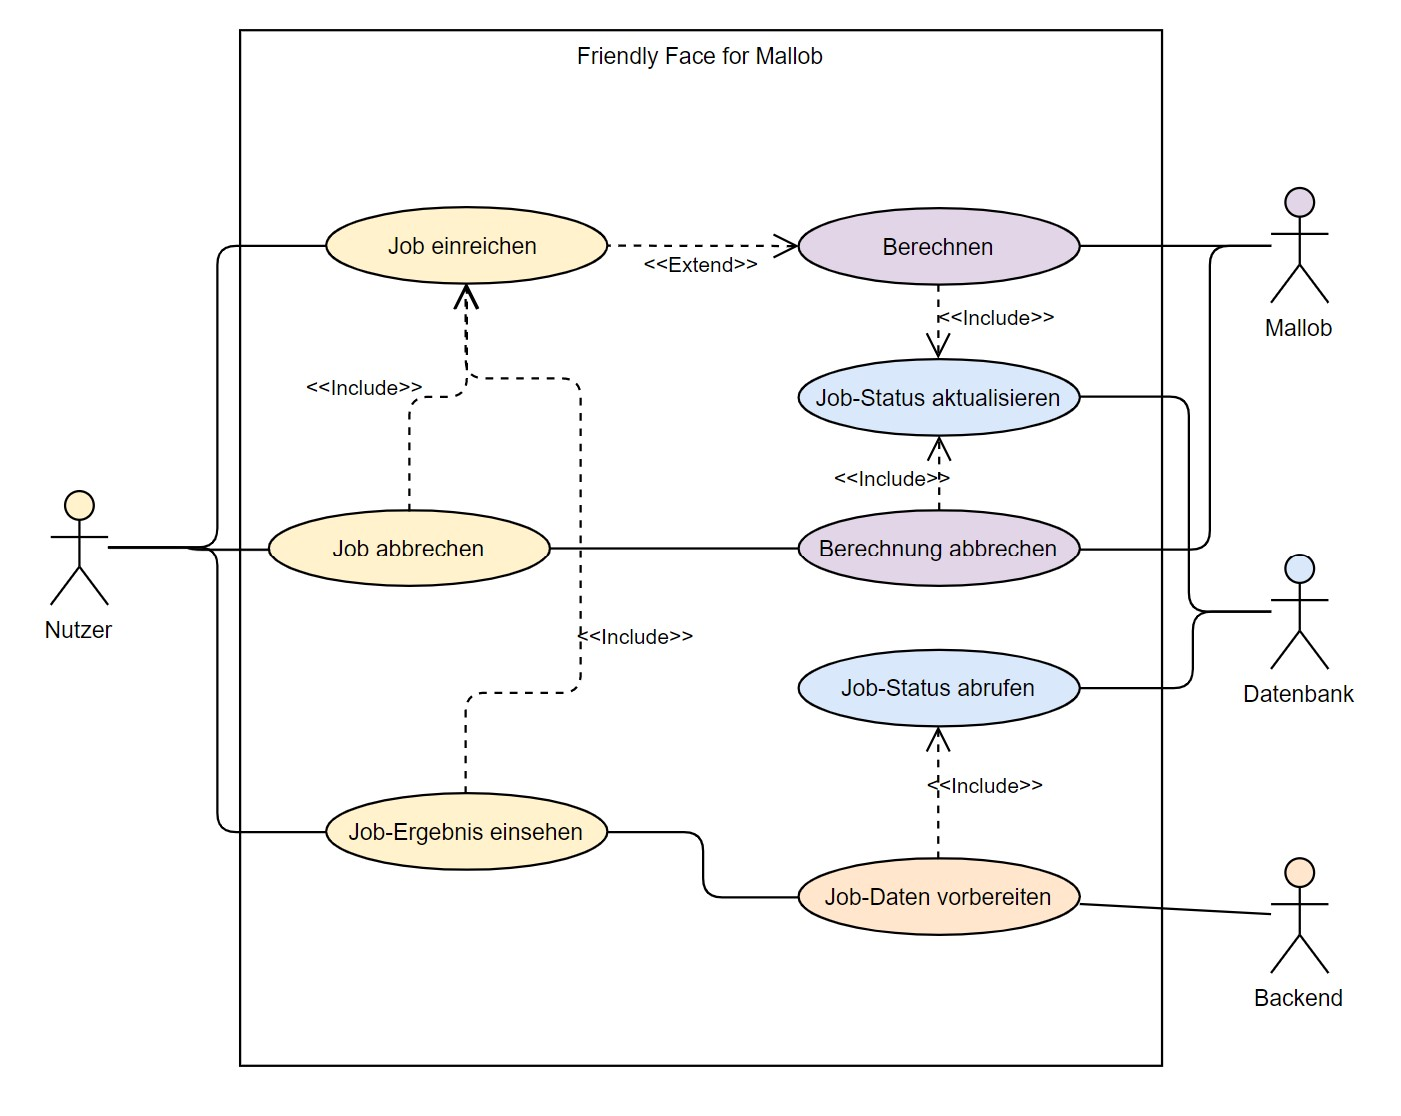
\includegraphics[width=\textwidth]{images-interface/Submit-abort-view-screenshot.jpg}
    \caption{Einreichen, Abbrechen und Einsehen von Jobs}
\end{figure}

Reicht ein Nutzer ein Job ein, so wird dieser (je nach Konfiguration) von Mallob bearbeitet. Mallob gibt dabei Rückmeldung über den Job-Status, also entweder das Ergebnis des Jobs, oder ob ein Fehler aufgetreten ist. Dieser Status wird in der Datenbank gespeichert. \\
Ein Nutzer kann die Bearbeitung eines Jobs, der gerade von Mallob berechnet wird, abbrechen. Die berechneten Zwischenergebnisse werden dann gespeichert und können später abgerufen werden. \\
Möchte ein Nutzer einen Job einsehen, so ist es wichtig das dieser bereits eingereicht wurde. Um ein Job einsehen zu können werden zunächst die angeforderten Job-Daten aus der Datenbank geholt und dann vorbereitet an den Nutzer geschickt.



%\begin{center}
%    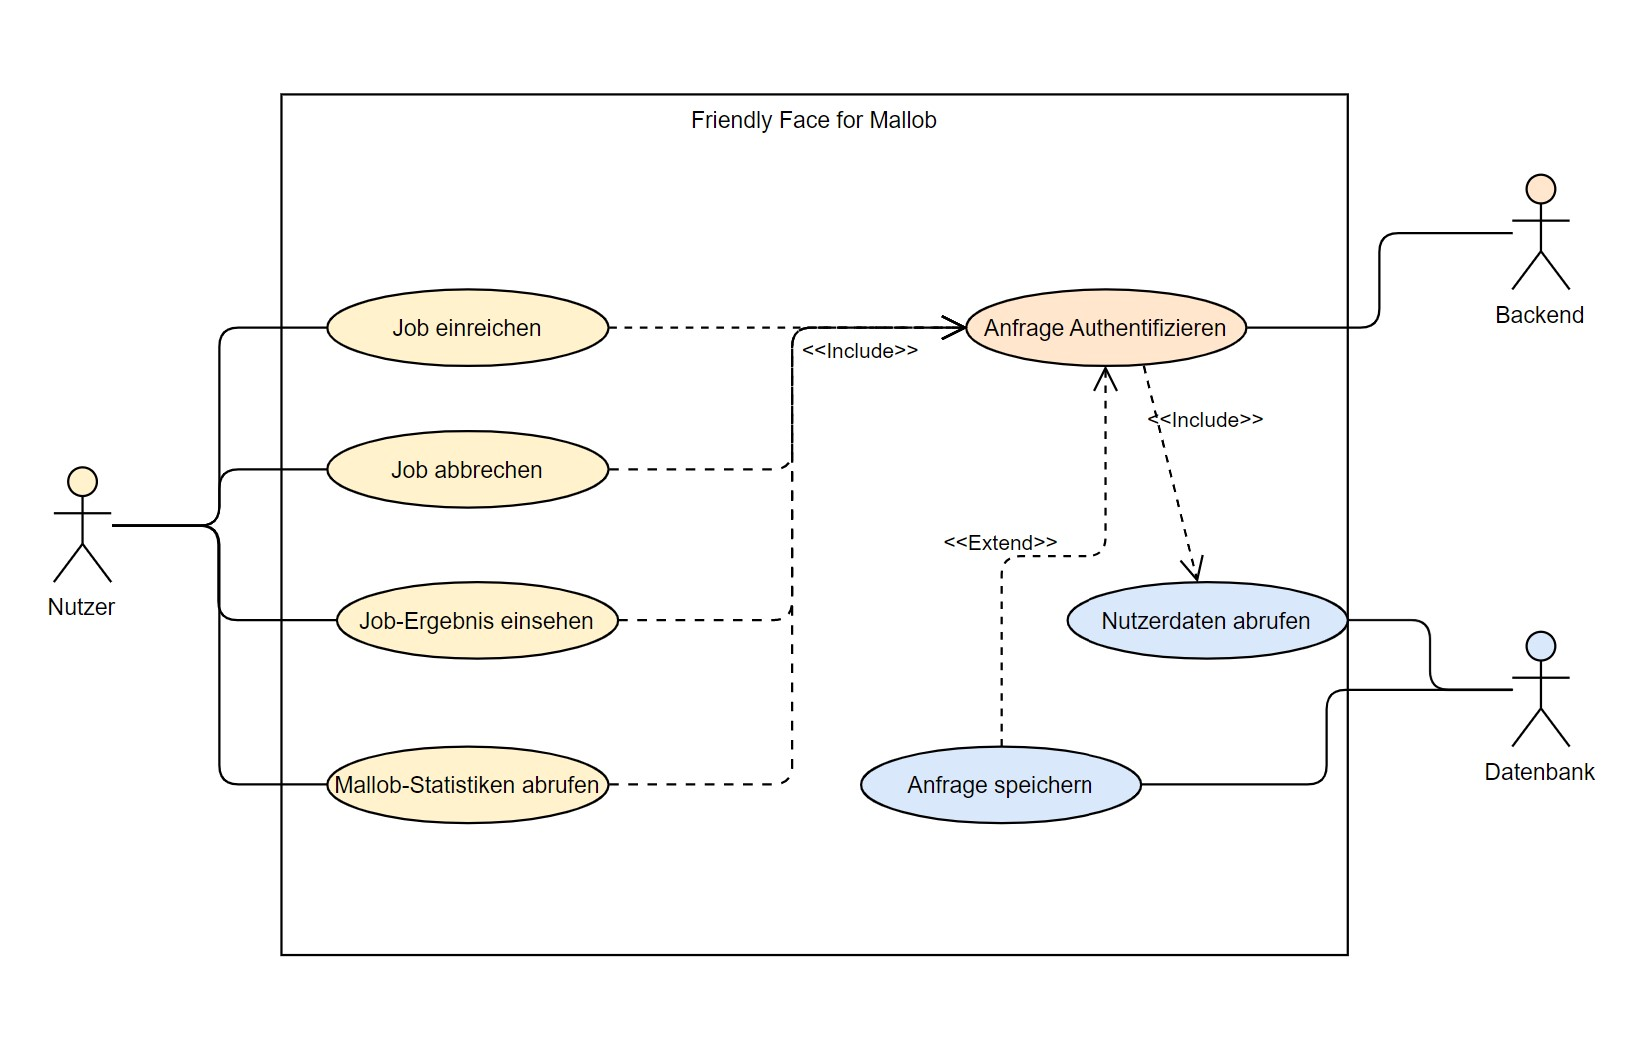
\includegraphics[scale=0.6]{images-interface/Request_authntification_screenshot.jpg} \\
%    Anwendungsfalldiagramm 2: Authentifizierung von API-Requests
%\end{center}


\begin{figure}[H]
    \centering
    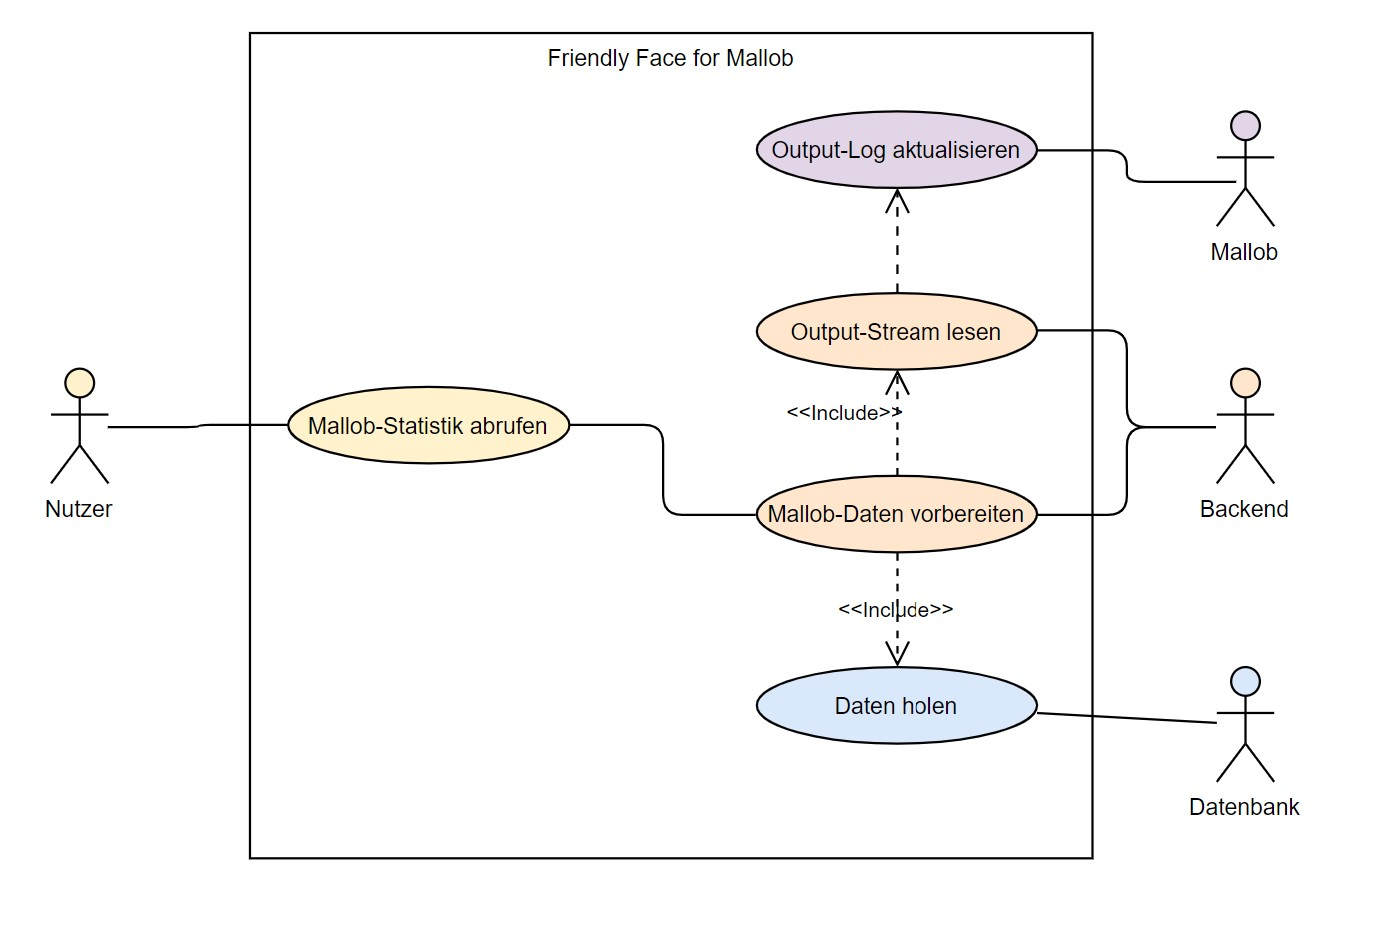
\includegraphics[width=\textwidth]{images-interface/Mallob-visualisierung.jpg}
    \caption{Mallob-Statistiken abrufen}
\end{figure}
Möchte ein Nutzer Mallob-Statisteiken abrufen, so holt das System bereits vergangene Events aus der Datenbank um hieraus Statistiken sowie Visualisierung vorzubereiten. Des weiteren wird live der Output-Log von Mallob ausgelesen, um Echtzeitdiagnostik sowie Echtzeit-Visualisierung für den Nutzer anzubieten. 


\pagebreak

\subsection{Aktivitätsdiagramme}
\begin{figure}[H]
    \centering
    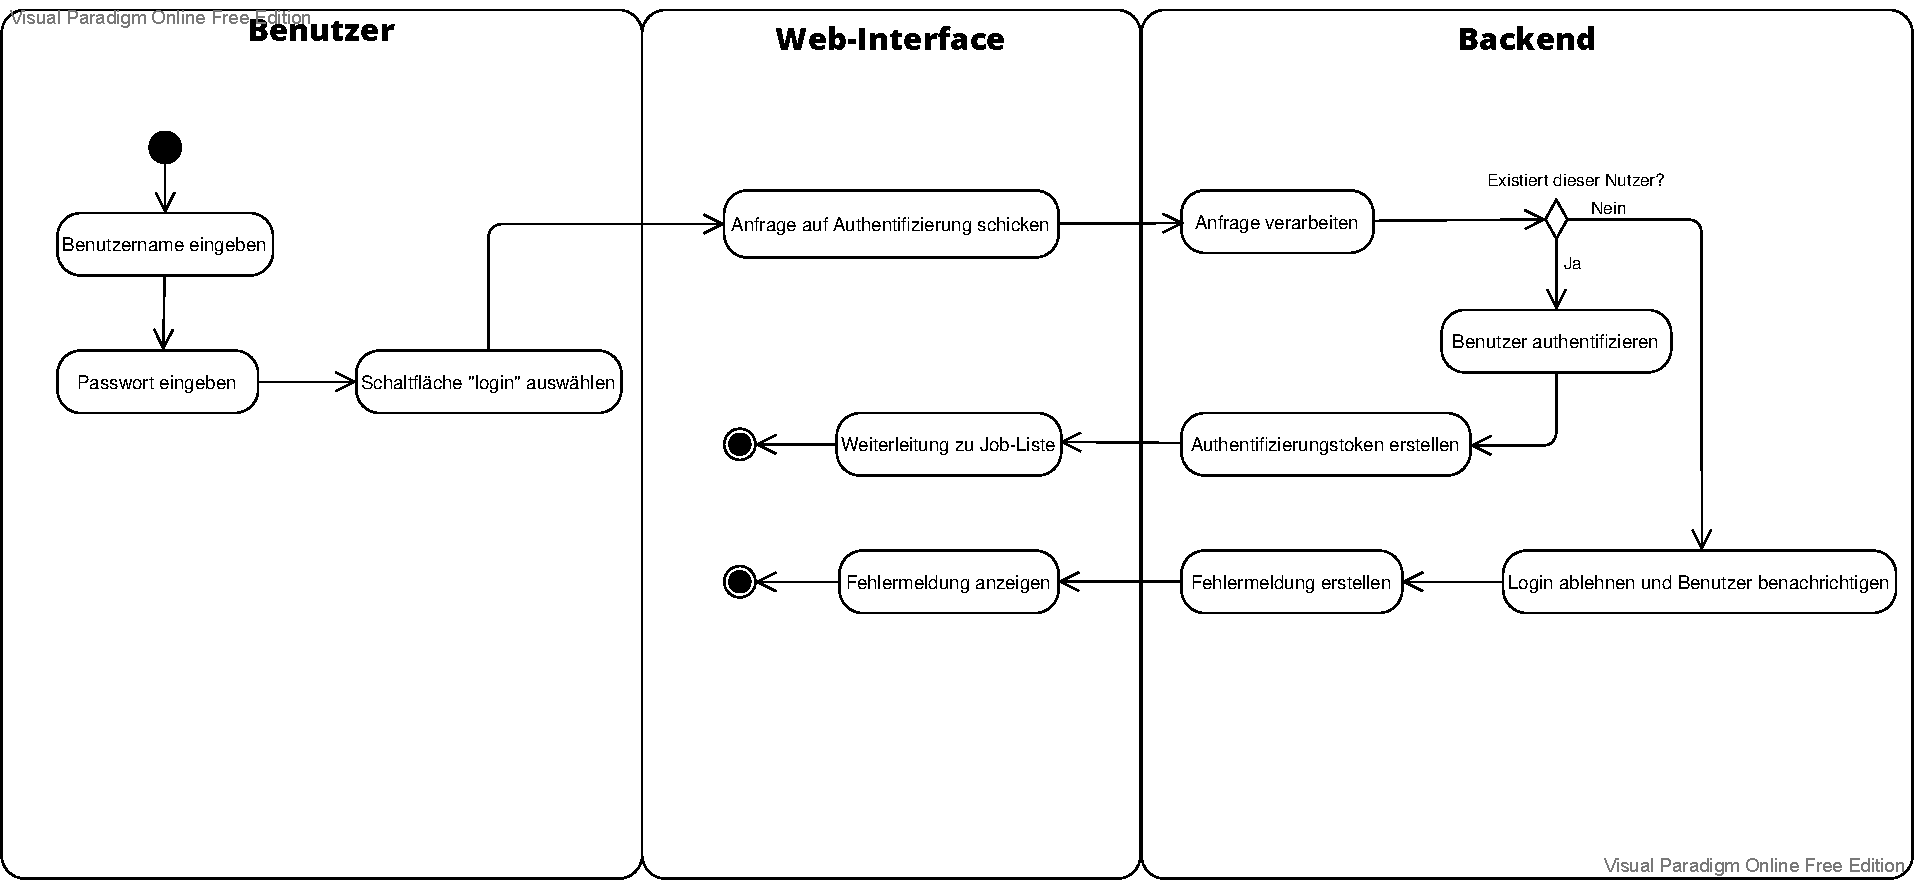
\includegraphics[width=\textwidth]{images-interface/Anmelden_Aktivitaetsdiagramm.pdf}
    \caption{Anmeldung im System über das Web-Interface}
    \label{fig:login_activity}
    
\end{figure}

\begin{figure}[H]
    \centering
    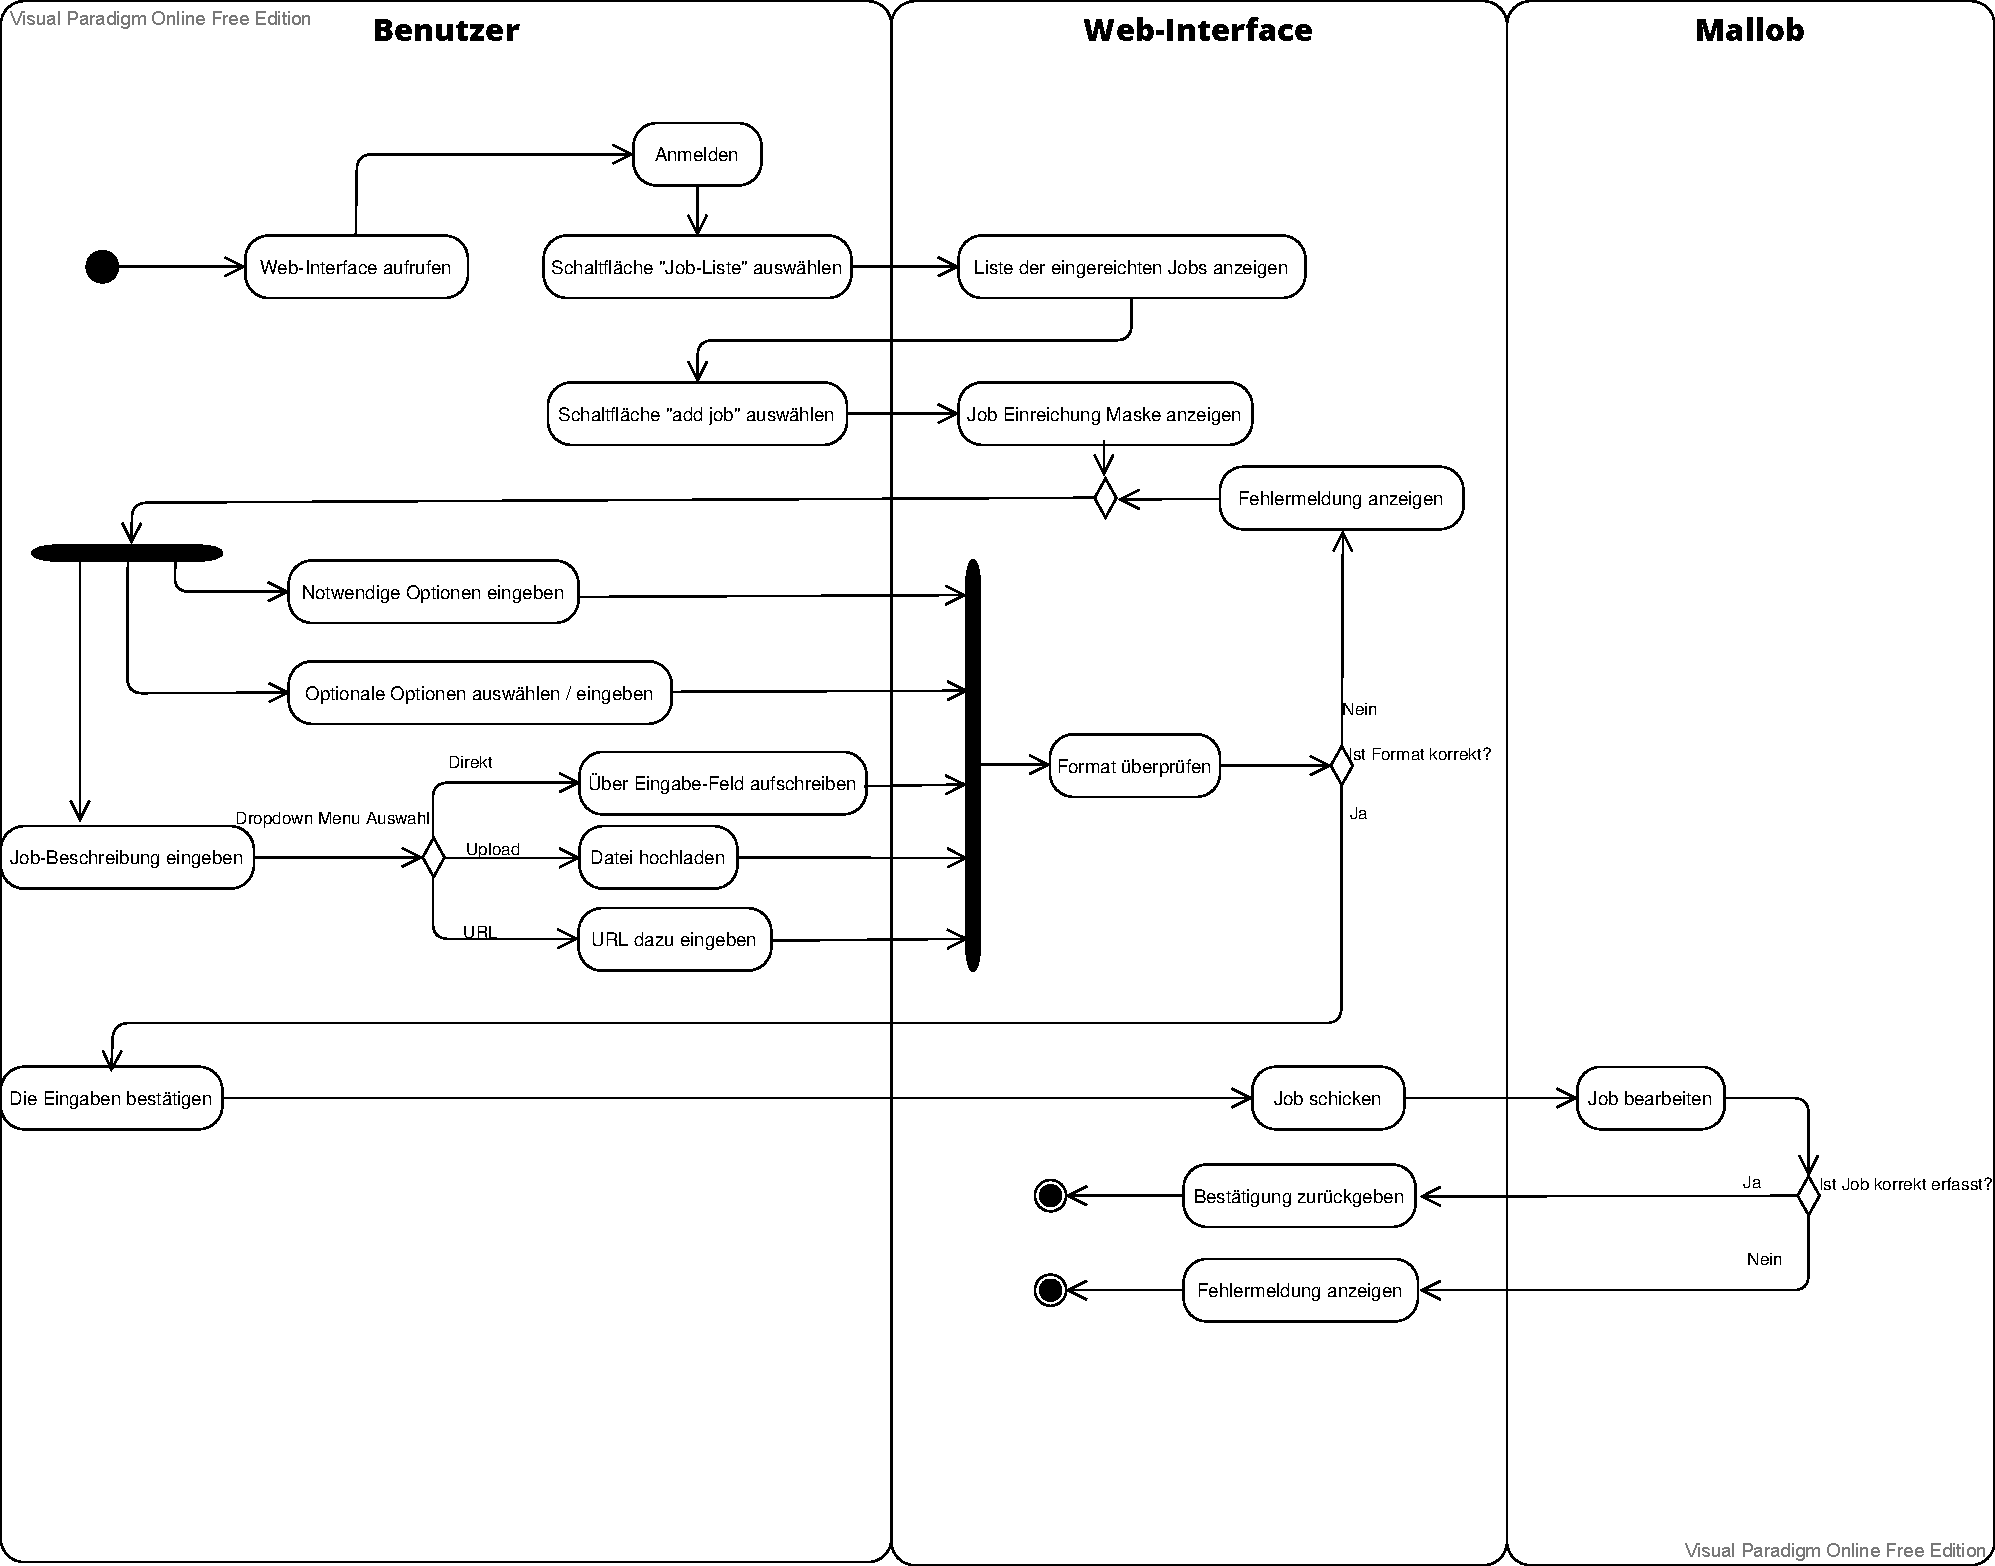
\includegraphics[width=\textwidth]{images-interface/Job_einreichen_Aktivitaetsdiagramm.pdf}
    \caption{Einreichen eines Jobs über das Web-Interface}
\end{figure}

\begin{figure}[H]
    \centering
    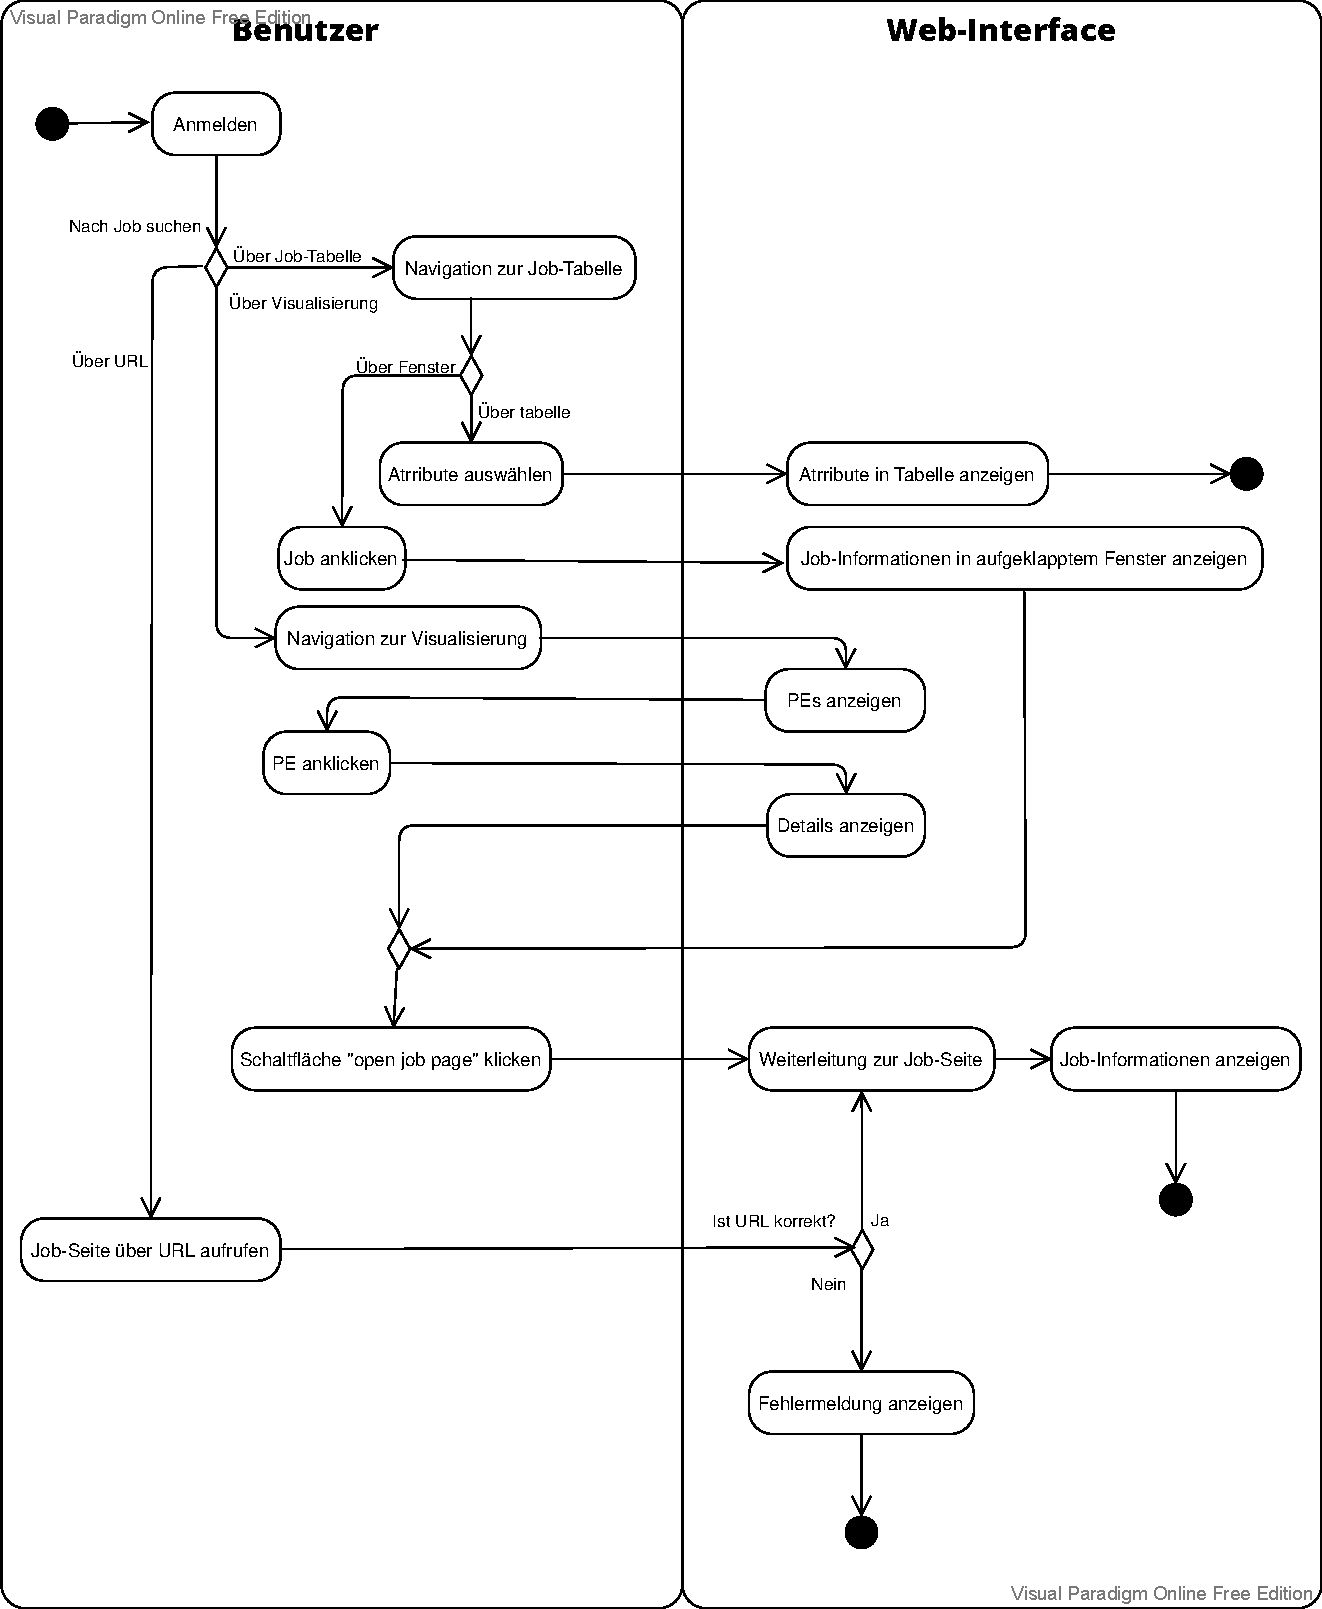
\includegraphics[width=\textwidth]{images-interface/get_infos.pdf}
    \caption{Einsehen von Job-Informationen}
\end{figure}